\chapter{Job Ads}
\label{chap:jobads}

Suppose that our company web site will soon feature a new set of job ads.
The old way of typing directly into html pages has worn through.  In this
chapter, we'll build the foundation for the new system, by creating a web
app to enter and update job and position descriptions.  [Our shop actually
feeds job ads to our public facing web server via RSS from an internal
Gantry bulletin board app.]

The key features of the application from a pedogogical point of view are
these: many-to-many relationships between database tables, limiting who
can access the app (auth), and creative CRUD where a single page submission
leads to activity in multiple tables.

\section{Step One: Creating Jobs and Their Skills}

Eventually the powers that be want a complete on-line way to manage job
descriptions, position announcements, and to track applications for those
positions.

While the plans for the app are ambitious, we are starting modestly,
with three main concepts: job descriptions, skills, and positions.  Each
of these will be a table in the database, but we need one more.  Since
the relationship between skills and job descriptions is many-to-many, we
need a table to join them.

A job description will have a title and a general description, like
``Cleaner'' - ``Keeps the building sparkling.''  There could be quite
a few people with that job description, each one is in a position.
But, for our purposes we will use `position' as short hand for `position
announcement.'  These let the world know that we are looking to expand our
fast-paced, team-oriented environment with a number of highly motivated
self-starters.  Skills are things that people are able to do, like
``coffee making.''  But we will probably stretch the term skill to
include things like ``valid driver's license and clean driving record.''

We're ready to write the vast bulk of the app.  Let's start with
tentmaker:

\begin{verbatim}
tentmaker -n JobAd 'job<->skill position->job'
\end{verbatim}

With the structure in place, use tentmaker to make the normal changes.
To begin, change the name of the ident field in the job table to `title.'
For once, `description' can stay as is.  Then, add fields for
travel percent, on site, and time percent.

The last two new fields will require the user to choose from a list of
options.  In the last chapter we had a similar problem with the invoice
status.  There, I chose to use a table to specify the statuses.  We
could do the same here.  But, in the interest of diverse solutions (and to
save data model complexity), let's let the app front end control the choices.

Start by choosing \verb+on_site+ from the `Edit Field:' selection
list.  That will reveal form elements which control all aspects of the
field and should look something like Figure \ref{fig:fieldedit1}.

\begin{figure}
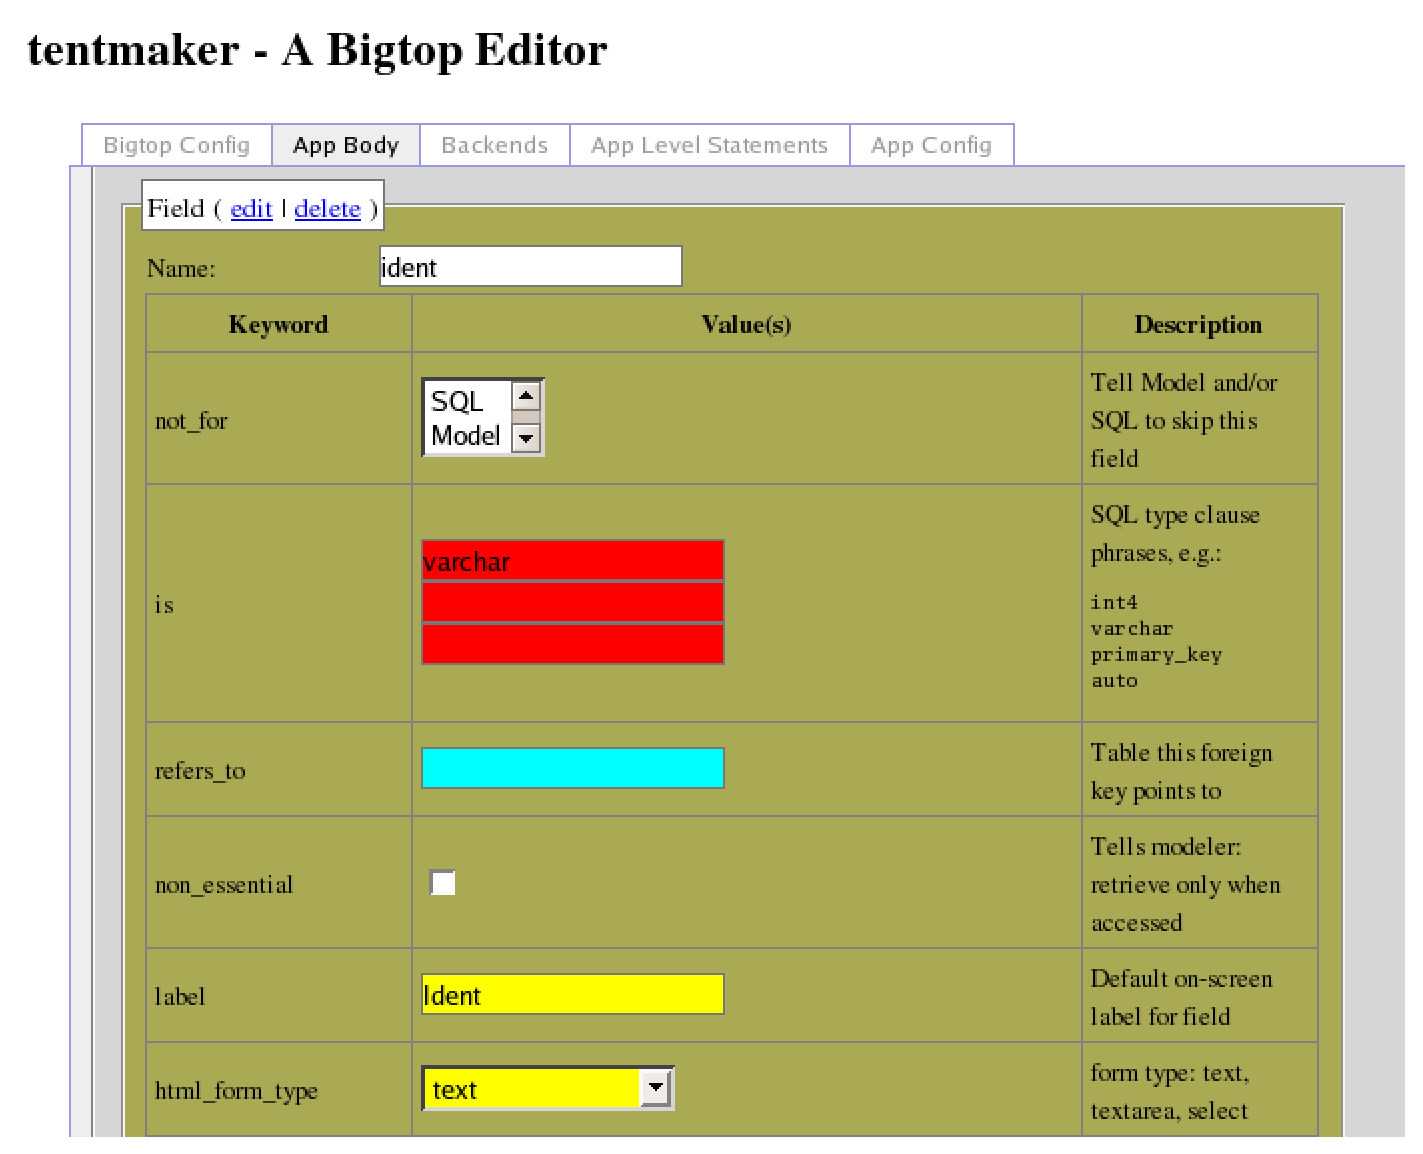
\includegraphics[width=6in]{fieldedit}
\caption{Full field edit form (same as Figure \ref{fig:fieldedit}).}
\label{fig:fieldedit}
\end{figure}

Some of these are represented in the quick edit table, but not
the ones we need to set.  First, choose `select' from the
\verb+html_form_type+ drop down menu.  Then, scroll down until you see
\verb+html_form_options+.  Enter the following:

\begin{tabular}{l|l}
Label               & Database Value    \\
\hline
On-Site             & onsite            \\
Partial Telecommute & parttele          \\
Telecommute         & tele              \\
\end{tabular}

Do the same things for \verb+time_percent+.  First, choose
\verb+html_form_type+ select.  Then, enter options like these:

\begin{tabular}{l|l}
Label               & Database Value    \\
\hline
Full Time           & fulltime          \\
Part Time           & parttime          \\
Contract            & contract          \\
\end{tabular}

This technique gives us data integrity, so long as all database access
is through the app.  But it saves us two tables in this case.

That's all we need to do for the job table.  The skill table is the rare
bird which can use the default fields.  So, let's edit the position
table.  The position description will be formed from the job description
and skills list, so we should delete that field.  To delete a field,
first select it from the `Edit Field:' drop down.  Then click delete
in the legend of the field set that surrounds the full edit form.
Finally, click `Ok' in response to `Are you sure you want to delete' in
the confirmation pop-up.  (Deleting is one thing that is always easier
in a text editor, but switching back and forth can itself be tedious.)

We need to add fields to this table.  Mine are called \verb+n_openings+,
\verb+location+, \verb+closes+, \verb+boss+, and \verb+pay+.  Only two
of them need more work.  Make the SQL Type for \verb+closes+ `date.'
Then make the SQL Type for \verb+n_openings+ int4 and add a constraint to
it: \verb_qr{^\d+$}_.  This will make sure the number is positive.  Well,
it does allow zero, feel free to craft a better regex.

This is enough to put in the job descriptions, the position announcements,
and the skills.  But it doesn't provide a way to link the skills to their
job descriptions.  And, as we'll see later, it doesn't meet management's
full requirement set.  It will serve as our starting point, so save the
bigtop file and stop tentmaker.

Since we didn't start with bigtop in new mode, we need to do the initial
build of the app:

\begin{verbatim}
bigtop -c jobad.bigtop all
\end{verbatim}

This creates the build directory JobAd, which you should change to.
You could spell out -c as --create.  Now, it is probably a good idea to
edit the bigtop file in \verb+docs/jobad.bigtop+ so that its Init Std
config block looks like this:

\begin{verbatim}
    Init Std { no_gen 1; }
\end{verbatim}

In new mode, bigtop does this for us.  It tells bigtop not to build any
of the Init Std files.  These include MANIFEST, which would be safe to
update.  But they also include Change, which should remain, well unchanged.
You could also be more specific, picking the files you want to leave alone:

\begin{verbatim}
    Init Std { Changes no_gen; }
\end{verbatim}

You could also make those choices on the `Backends' tab in tentmaker.
Finally, we are ready to begin customizing the application, starting
with initial user objections.

\section{Authorizing Users}

Upon seeing the original data model from the last section, management
immediately asked us to track logged in users and what they did to the data.
This is a two fold request.  First, have a login scheme so only certain
people can access the app.  Second, when they are in the app, track what
they do in a change log.  This section tackles the first request, the next
section the second.

There are many ways to authorize users in a web app.  Gantry, can help you
do it, if you choose to use Apache basic auth.  This section explains how
to accept that help.  Always remember that Gantry is here to help you, if
you don't feel it is helping, it will gladly step out of the way.  When you
do use Gantry's auth scheme, you should run your server over SSL, keep it
behind a firewall, or both.

To understand Gantry's auth scheme, you need to understand a bit about
how our business uses Gantry.  We deliever many applications via the
web.  Most of them are served to employees behind our firewall.  Therefore,
we want all the apps to use the same user names and passwords.  In fact,
we only want to store those once.  So, we have a master auth database
where everyone's login credentials are stored.  Ideally, each app uses
it for validation.  In reality there are exceptions, with some apps
periodically pulling updates from master auth into their own auth tables.
Here, I will focus on the ideal.  Thus, there will be two databases:
jobad.db and auth.db.  The second can easily be shared across an
organization's apps (we even share ours with apps written with the
prior version of Gantry, which never left the shop).  I must admit that
this approach also simplifies the following discussion.  It is harder to
use Gantry's auth scheme when the auth tables are embedded in the app's
database, not impossible, just harder.

To create your auth database, use a schema file that comes in the
gantry distribution: docs/authschema.sql (Postgres) or docs/authschema.sqlite.
As we will see below, Gantry provides controllers for maintaining the
data in the database once you build it.

Here is a tour of the auth data model.  The key table is \verb+auth_users+.
It has the user name, real name, and password for each user.  The other
tables are tied to it in one way or another.

In addition to individual rights, many apps, including this one, have group
requirements.  Suppose that any valid user may update or add job descriptions
and skills, but only HR can create and manage positions.  This leads to one
group: HR.  In addition, we might want an admin group to manage the
\verb+auth_users+ table.  For now the HR group members will be allowed to
do that.  Gantry auth uses \verb+auth_groups+ to name the groups and
\verb+auth_group_members+ to enroll users in them.  There is also an ip based
auth scheme, but we don't need to think about that for this app.

We don't need to add tables or controllers to our bigtop file for the
auth scheme, but we do need to add some conf to make it happen.  First,
I'll use \verb+mod_perl+.  You could also use CGI, but not the stand alone
server, which does not understand the HTTP auth protocol.





This is enough to put in the job descriptions, the position announcements,
and the skills.  But it doesn't provide a way to link the skills to their
job descriptions.  And, as we're about to see, it doesn't meet management's
full requirement set.

This bigtop file assumes that you are going to incorporate the auth tables
into your app's regular database.  But, you could change that simply by
altering the DBI connection string for \verb+auth_dbconn+ in the app level
config block.

The best way to set up the auth part of your database is to use the schema
provided in the docs directory of the Gantry distribution, though that will
take a bit of translation if you don't use Postgres.

Once you have the database set up, you can easily turn on location based
auth by user or group in your apache conf.

\section{Tracking User Changes}

\begin{verbatim}
changelog
    id
    user_id
    descr
\end{verbatim}

%\begin{figure}
%\includegraphics[width=6in]{name}
%\caption{Caption.}
%\label{fig:name}
%\end{figure}
